\subsection{NonUniformHexahedronFEMForceFieldAndMass}
\graphicspath{{../modules/}}  % to include images


\subsubsection{Concepts}

This force field implement the article :

\begin{verbatim}
      @InProceedings{NPF06,
      author       = "Nesme, Matthieu and Payan, Yohan and Faure, Fran\c{c}ois",
      title        = "Animating Shapes at Arbitrary Resolution with Non-Uniform Stiffness",
      booktitle    = "Eurographics Workshop in Virtual Reality Interaction and Physical Simulation (VRIPHYS)",
      month        = "nov",
      year         = "2006",
      organization = "Eurographics",
      address      = "Madrid",
      url          = "http://www-evasion.imag.fr/Publications/2006/NPF06"}
 \end{verbatim}
 
 
 
The basic idea, illustrated in figure \ref{fig:condensation}, is :


\begin{figure}
\begin{center}
	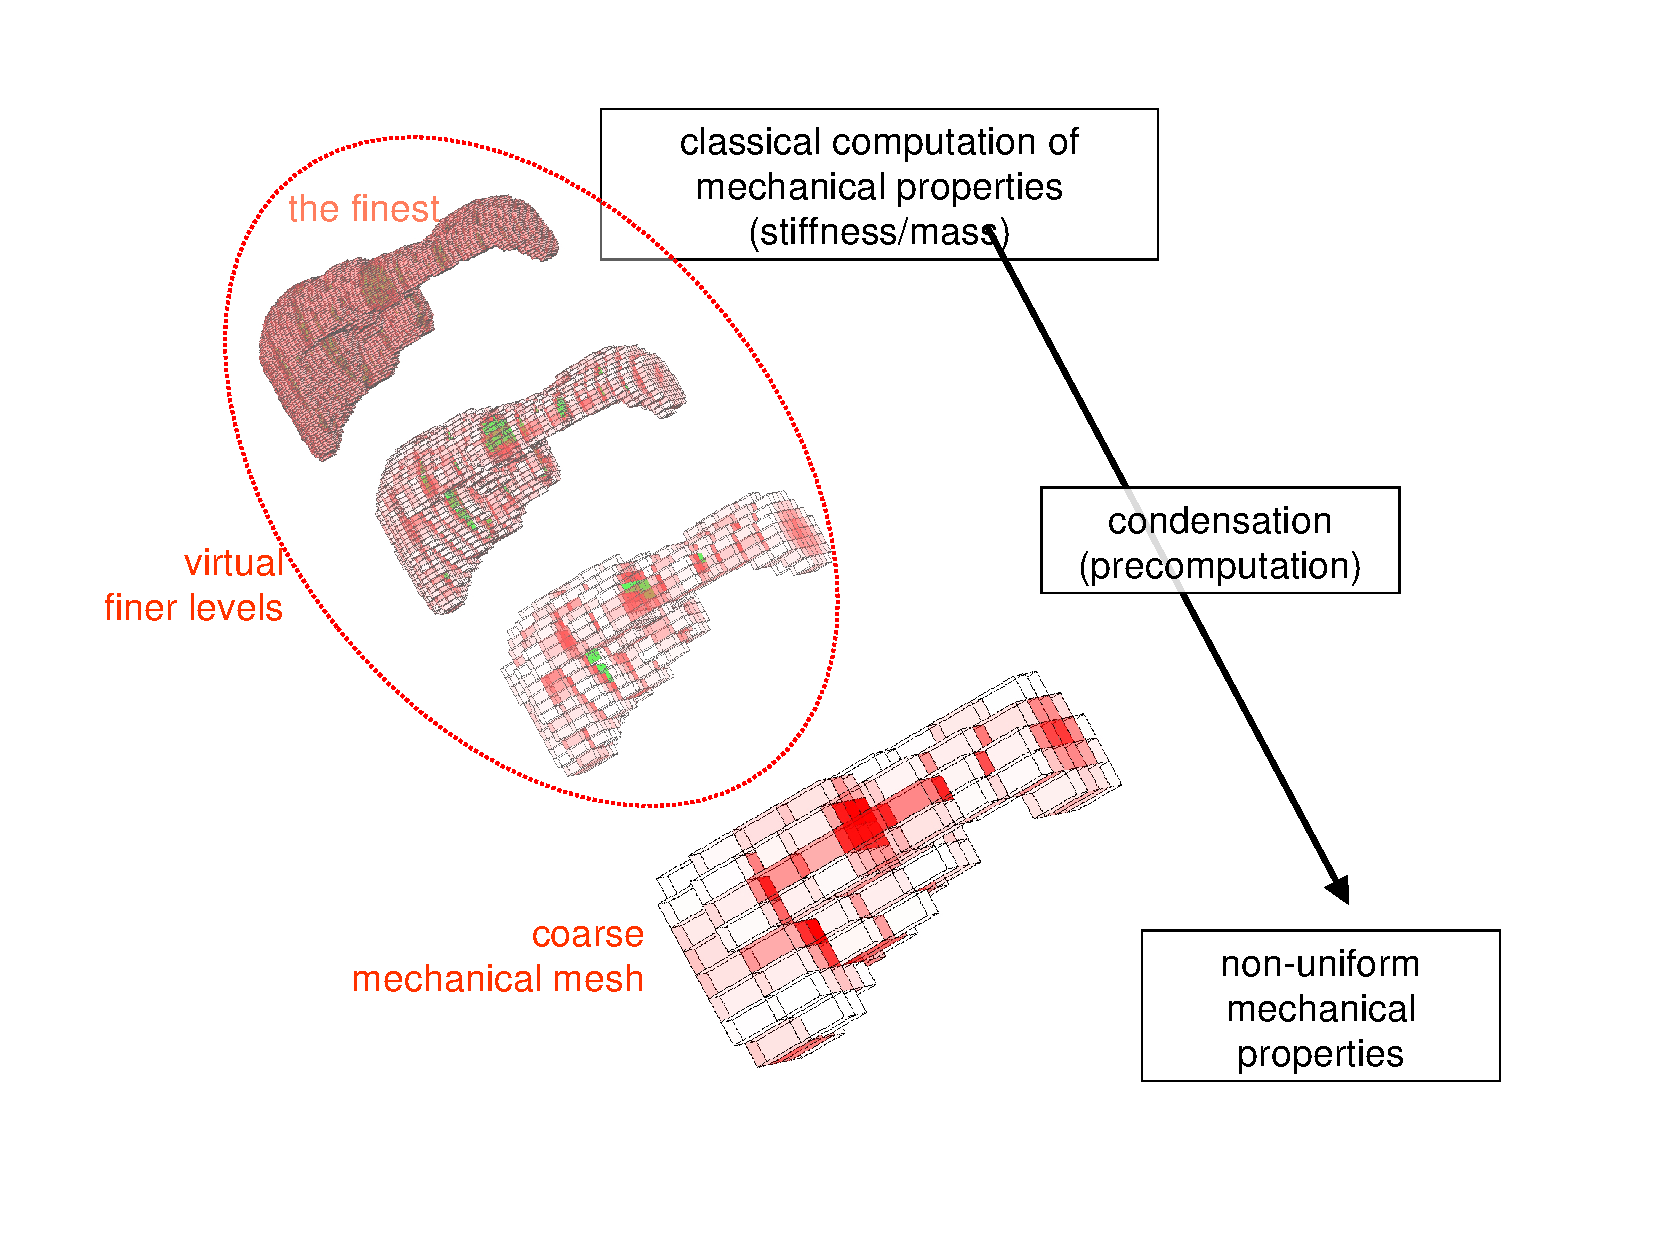
\includegraphics[width=\linewidth]{forcefield/nonUniformHexahedron/condensation.pdf}
\end{center}
	\caption{The condensation principle.}
	\label{fig:condensation}
\end{figure}



\begin{itemize}
\item the use of finer virtual levels of SparseGrid
\item the computation of classical mechanical matrices (mass and stiffness) at the finest resolution and the condensation of theses matrices to the current coarse mechanical resolution
\end{itemize}


\textbf{Warning} : actually the NonUniformHexahedronFEMForceFieldAndMass is only working with SparseGridTopology, and need enough finer virtual levels to compute the condensation. 

\subsubsection{Data Fields}

\begin{itemize}
\item From HexahedronFEMForceFieldAndMass
	\begin{itemize}
	\item method (char) : large/polar, the corotationnal method (default = large)
	\item poissonRatio, youngModulus, density (float) : mechanical properties (density = volumetric mass in english $kg.m^{-3}$)
	\item assembling (bool) : assembling the global system matrix ? (default = false)
	\end{itemize}
\item Specific to NonUniformHexahedronFEMForceFieldAndMass
	\begin{itemize}
	\item nbVirtualFinerLevels (int) : how many finer virtual levels are employed in the condensation stage ? (default = 0)
	\end{itemize}
\item A hack on masses (for debugging)
		\begin{itemize}
	\item useMass (bool) : are the condensated mass matrices are used ? (if not, scalar masses concentrated on particles are used) (default = 0)
	\item totalMass (float) : if useMass=false, the scalar mass of the object
	\end{itemize}
\end{itemize}


\subsubsection{Example}



\begin{verbatim}

<Node name="non uniform">
   <Object type="SparseGrid"
                   n="4 4 4"
                   filename="mesh/mymesh.obj"
                   nbVirtualFinerLevels="2"  />
   <Object type="MechanicalObject"/>
   <Object type="NonUniformHexahedronFEMForceFieldAndMass"
                   nbVirtualFinerLevels="2"
                   youngModulus="20000"
                   poissonRatio="0.3"
                   density="10" />
</Node>

\end{verbatim}

\textbf{Important} : note that the SparseGrid has nbVirtualFinerLevels=2 in order to built enough finer virtual levels. This SparseGrid$->$nbVirtualFinerLevels has to be greater or equal to the NonUniformHexahedronFEMForceFieldAndMass$->$nbVirtualFinerLevels.
\\

A more complex example can be found in : examples/Components/forcefield/NonUniformHexahedronFEMForceFieldAndMass.scn where a comparison with a classical HexahedronFEMForceFieldAndMassForceField is done.

